\documentclass{sigchi-ext}
% Please be sure that you have the dependencies (i.e., additional
% LaTeX packages) to compile this example.
\usepackage[T1]{fontenc}
\usepackage{textcomp}
\usepackage[scaled=.92]{helvet} % for proper fonts
\usepackage{graphicx} % for EPS use the graphics package instead
\usepackage{balance}  % for useful for balancing the last columns
\usepackage{booktabs} % for pretty table rules
\usepackage{ccicons}  % for Creative Commons citation icons
\usepackage{ragged2e} % for tighter hyphenation

% Some optional stuff you might like/need.
% \usepackage{marginnote} 
% \usepackage[shortlabels]{enumitem}
% \usepackage{paralist}
% \usepackage[utf8]{inputenc} % for a UTF8 editor only

%% EXAMPLE BEGIN -- HOW TO OVERRIDE THE DEFAULT COPYRIGHT STRIP --
% \copyrightinfo{Permission to make digital or hard copies of all or
% part of this work for personal or classroom use is granted without
% fee provided that copies are not made or distributed for profit or
% commercial advantage and that copies bear this notice and the full
% citation on the first page. Copyrights for components of this work
% owned by others than ACM must be honored. Abstracting with credit is
% permitted. To copy otherwise, or republish, to post on servers or to
% redistribute to lists, requires prior specific permission and/or a
% fee. Request permissions from permissions@acm.org.\\
% {\emph{CHI'14}}, April 26--May 1, 2014, Toronto, Canada. \\
% Copyright \copyright~2014 ACM ISBN/14/04...\$15.00. \\
% DOI string from ACM form confirmation}
%% EXAMPLE END

% Paper metadata (use plain text, for PDF inclusion and later
% re-using, if desired).  Use \emtpyauthor when submitting for review
% so you remain anonymous.
\def\plaintitle{Constructing Identity and Local Community through Tangible Exploration} \def\plainauthor{Diego Salvatierra, Po Tsui}
\def\emptyauthor{}
\def\plainkeywords{Identity construction environment; child-computer interaction; youth; education; tangible user interfaces}
\def\plaingeneralterms{Documentation, Standardization}

\title{Constructing Identity and Local Community through Tangible Exploration}

\numberofauthors{2}
% Notice how author names are alternately typesetted to appear ordered
% in 2-column format; i.e., the first 4 autors on the first column and
% the other 4 auhors on the second column. Actually, it's up to you to
% strictly adhere to this author notation.
\author{%
  \alignauthor{%
    \textbf{Diego Salvatierra}\\
    \affaddr{Stanford University} \\
    \affaddr{Stanford, CA 94305, USA} \\
    \email{dsalva@stanford.edu} }\alignauthor{%
    \textbf{Po Tsui}\\
    \affaddr{Stanford University}\\
    \affaddr{Stanford, CA 94305, USA}\\
    \email{potsui@stanford.edu} } }

% Make sure hyperref comes last of your loaded packages, to give it a
% fighting chance of not being over-written, since its job is to
% redefine many LaTeX commands.
\definecolor{linkColor}{RGB}{6,125,233}
\hypersetup{%
  pdftitle={\plaintitle},
%  pdfauthor={\plainauthor},
  pdfauthor={\emptyauthor},
  pdfkeywords={\plainkeywords},
  bookmarksnumbered,
  pdfstartview={FitH},
  colorlinks,
  citecolor=black,
  filecolor=black,
  linkcolor=black,
  urlcolor=linkColor,
  breaklinks=true,
}

% \reversemarginpar%

\begin{document}

%% For the camera ready, use the commands provided by the ACM in the Permission Release Form.
%\CopyrightYear{2007}
%\setcopyright{rightsretained}
%\conferenceinfo{WOODSTOCK}{'97 El Paso, Texas USA}
%\isbn{0-12345-67-8/90/01}
%\doi{http://dx.doi.org/10.1145/2858036.2858119}
%% Then override the default copyright message with the \acmcopyright command.
%\copyrightinfo{\acmcopyright}

\maketitle

% Uncomment to disable hyphenation (not recommended)
% https://twitter.com/anjirokhan/status/546046683331973120
\RaggedRight{} 

% Do not change the page size or page settings.
\begin{abstract}
\end{abstract}

\keywords{\plainkeywords}

\category{H.5.m}{Information interfaces and presentation (e.g.,
  HCI)}{Miscellaneous}\category{See}{\url{http://acm.org/about/class/1998/}}{for
  full list of ACM classifiers. This section is required.}

\section{Introduction}

\section{Theoretical and Design Framework}
Rooted primarily in the theories of critical pedagogy and constructionism, our project aims to achieve, through a tangible user interface (TUI) as per Papert's "objects-to-think-with" (Papert 11), Freire's idea that learners should become aware of their world and its social and political conditions - through what Freire calls "a constant unveiling of reality" (Freire 81) - and their position within it. 

A key part of this reality includes the learner's surrounding communities and their own personal histories, which is the focus of our project. Additionally, Freire stresses the crucial component of "praxis," through which students not simply explore, but transform and construct the world. He recognizes that "reality is a process" (Freire 75); as such, students must come to understand that they are simultaneously part of this dynamic reality and in the position to change it. This is the process of conscientiza\c{c}\~{a}o. By allowing learners to construct personally significant places and events on a physical timeline and map, we aim to help students undergo the active and deliberate process of creating their reality.

Related to Freirean concepts of critical consciousness is identity construction; thus, we draw on the psychological theories of Erik Erikson (1962) for understanding how our target learners, middle- and high-school students, view themselves. Erikson describes the psychosocial crises that individuals experience in different stages of life. During the "identity vs. role confusion" stage experienced by adolescents, they feel "a sense of the irreversibility of significant events and an often urgent need to understand fully and quickly what kind of happenings in reality and in thought determine others, and why" (Erikson 16). In other words, adolescents seek historical frameworks, identities, and roles in which to make sense of who they are. Through our project, we aim to help them understand the events that, to quote Erikson, "determine others," and the historical events that have shaped themselves.

We do this on the foundations of Seymour Papert, primarily his concept of "objects-to-think-with" which help learners grasp certain abstract concepts through tangible means and share ideas in concrete ways to the world. Through our project, learners create physical representations of inner memories of past events and perceptions of their surround. In such a way, the TUI becomes an object for students to reflect upon their lives and their communities, and to share them publicly to the world in a novel way.

This builds on the concept of restructurations, as put forward by Wilensky and Papert (2010), which are new symbols and structures of knowledge that make it possible for learners to achieve previously difficult tasks. Our project is a restructuration of the existing means of storytelling of one's life history, which most commonly exist today as written and oral narratives. We introduce an autotopography which allows students to more easily share the story of their life and their community, with multiple entry points for those without considerable writing or artistic skills in other contexts. This approach also allows for a sweeping non-strictly-linear view through which macro-level patterns and insights could emerge, which abides by Wilensky's power principle.

The United States, like many other countries, suffers from high segregation in schools by race and class. As shown in fig. 1, the Bay Area is not immune from these dynamics. As our project help students become aware of the lived experiences of others in nearby communities, it is worth referring to studies that demonstrate how one can bridge social divides among different school communities. Lopez and Nastasi (2012) share their experience with a project that brought together youth from suburban and urban school districts. Students from different districts shared conversations on their own identities, followed by a collaborative project on how to improve their community. The authors found that "when curriculum and pedagogy help students to understand their own identities, the identities of their peers, and methods for collaboration, students are prepared for democratic participation" (Lopez and Nastasi 155). Although our project does not yet replicate the aforementioned methods of collaboration, we facilitate the first two pedagogical components put forward by these authors: helping students understand their own identities and those of their peers.

\begin{figure}
  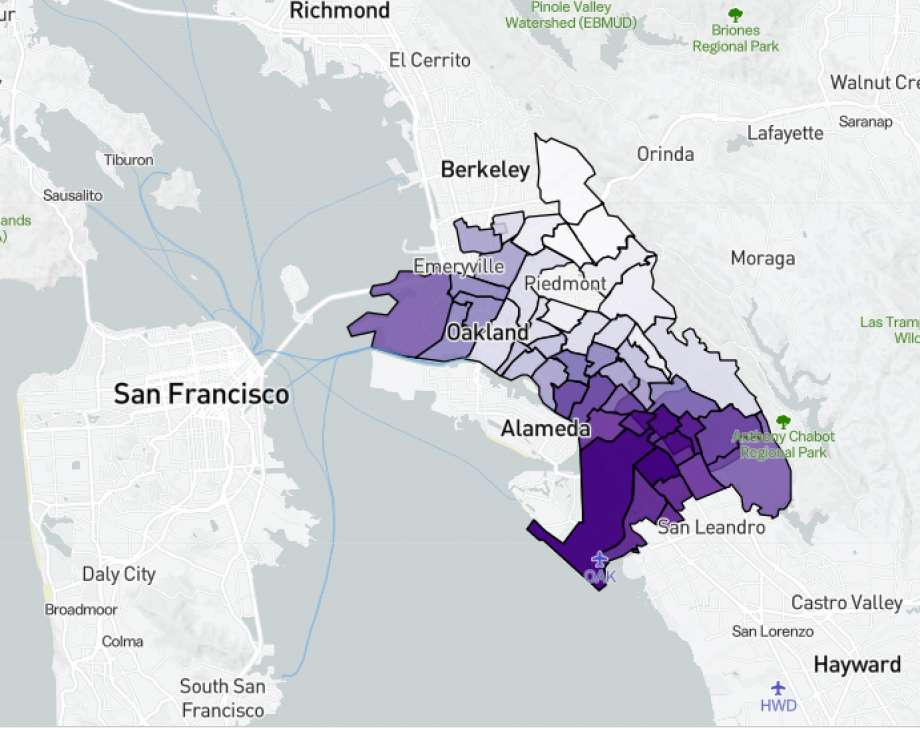
\includegraphics[width=0.9\columnwidth]{figures/map}
  \caption{School segregation in the Bay Area. Source: Vox, \textit{We can draw school zones to make classrooms less segregated. This is how well your district does.} 2018.}~\label{fig:sample}
\end{figure}

\section{Identity Construction Environments}

Marina Umaschi Bers (2009) has conducted extensive work on what she terms "Identity Construction Environments" (ICE), which are "technological tools purposefully designed to afford opportunities for exploring identity and engaging in reflection and discussion about personal and moral values" (368). We abide by the five principles she puts forth, which involve purposeful design to help young people learn about and construct their identity through community, storytelling, and dynamic objects representing the self.

We study Zora, a "three dimensional multi-user virtual environment that engages learners in the design of a graphical virtual city and its social organization" and the pivotal work behind Bers's ideas within this field. In this virtual environment, individuals create avatars of themselves, design their own living spaces, engage collaboratively in the construction and maintenance of their microcommunity. Zora also contains a "collaborative values dictionary" (406) through which individuals can explore their personal and moral values. 

Our project parallels some of the same elements found in Zora. Through our design, learners reflect on abstract histories, perceptions of their communities, and personal values in concrete ways through objects-to-think-with. The selection of what to display and share physically is an active process of self-reflection and construction of what is important to that individual. We make use of narrative therapy, which casts storytelling as the means through which construct ourselves and our identities.

However, Zora is situated within a virtual world and thus one level removed from the physical community in which the student lives and has developed personal history. We in contrast use the actual neighborhood as touchpoints for reflection and transforming action. We ground our users to their immediate surroundings and aim in Freirean fashion to lead to direct action upon the learner's world. By actively constructing and sharing their neighborhoods, students learn about the actual history of their immediate surrounding community and the lives of their peers. In doing so, we also differ from Zora's approach by placing an emphasis on the historicity of the individual and the community. We aim for learners to make sense of their own lived experiences and recognize themselves in the context of their community and family history, as standing on the backs of their ancestors. The design allows for users to view their construction as one whole, through which macro-level insights can emerge. Finally, our tangible user interface embodies a harder constructionist approach, wherein the abstract are represented by physical objects to be touched and manipulated by the hand. The physical placement of three-dimensional markers on our TUI map represents not only the physical construction of an individual's identity, but also a sociopolitical assertion of physical existence in the real world. 


\section{Acknowledgements}

%\balance{} 

\section{References}
\begin{enumerate}
\item Bers, Marina Umaschi. (2001) Identity Construction Environments: Developing Personal and Moral Values Through the Design of a Virtual City, The Journal of the Learning Sciences, 10:4, 365-415.

\item Bers, M. U. and Chau, C. (2006). Fostering Civic Engagement by Building a Virtual City. Journal of Computer-Mediated Communication, 11: 748–770.

\item Erikson, E. H. (1962). Youth: Fidelity and diversity. Daedalus, 5-27.

\item Freire, P. (2018). Pedagogy of the oppressed. Bloomsbury Publishing USA.

\item Lopez, G. E., \& Nastasi, A. W. (2012). Writing the Divide: High School Students Crossing Urban-Suburban Contexts. Equity \& Excellence in Education, 45(1), 138-158.	

\item Papert, S. (1980). Mindstorms: Children, computers, and powerful ideas. Basic Books, Inc.. Chicago

\item Wilensky, U., \& Papert, S. (2010). Restructurations: Reformulations of knowledge disciplines through new representational forms. Constructionism.
\end{enumerate}




%\bibliographystyle{SIGCHI-Reference-Format}
%\bibliography{sample}

\end{document}

%%% Local Variables:
%%% mode: latex
%%% TeX-master: t
%%% End:
